\documentclass{article}

\usepackage[polish]{babel}
\usepackage[T1]{fontenc}
\usepackage{tabularx}
\usepackage{amsfonts}
\usepackage{amsmath}
\usepackage{mathtools}
\usepackage{enumitem}
\usepackage{graphicx}
\usepackage{algpseudocode}

\begin{document}
    \begin{titlepage}
        \title{Algorymy metaheurystyczne}
        \author{Mateusz Chęciński, Mateusz Tofil}
        \maketitle
    \end{titlepage}

    \section{Wprowadzenie}

    Celem tej listy było zapoznanie się z algorytmem przeszukiwania z
    zabronieniami (z ang. Tabu search). 

    \section{Opis algortmu}

   Zaimplementowany algorytm jest mocno generyczny, mamy wiele opcji do wyboru.
   Na początku decydujemy, czy podajemy rozwiązanie początkowe 
   (lub np. funkcję heurystyczną, które takie wygeneruje), czy jest 
   ono losowe. Są także 3 możliwe warunki zakończenie: 
   liczba iteracji, liczba iteracji bez zmiany, czas.
   Algorytm w pętli generuje sąsiedztwo aktualnego rozwiązania
   (także są 3: swap, insert, invert). Następnie usuwa te rozwiązania,
   które są na liście tabu (jej długość także jest parametrem) i wybiera
   najlepsze z pozostałych. Oczywiście może zdarzyć się sytuacja, w której
   wszystkie rozwiązania są zabrobione. Wtedy mamy 5 opcji: 
   1) zakończenie algorytmu z aktualnym rozwiązaniem
   2) usuwanie rozwiązań z listy tabu dopóki jakieś będzie dozwolone
   3) powtórzenie algorytmu z innym roziwązaniem początkowym
   4) skorzystanie z kryterium aspiracji (pamięci długoterminowej), tzn.
   z zapamiętanego wcześniej rozwiązania, które było najlepsze, ale było zabronione,
   algorytm wykonuje nawrót
   5) generowanie nowych sąsiadów dopóki któryś będzie dozwolony
    

    \noindent Język programowania: Python 3.10

    \section{Porównanie otoczeń: insert, invert, swap}

    W celu zbadania jakie otoczenie jest najlepsze z
    powyższych 3, przeprowadziliśmy eksperymenty wywołując
    metode ze zmienionym parametrem początkowym. Wszystkie
    eksperymetry były przeprowadzone dla tej samej instacji
    wraz z tym samym rozwiązaniem początkowym.
    
    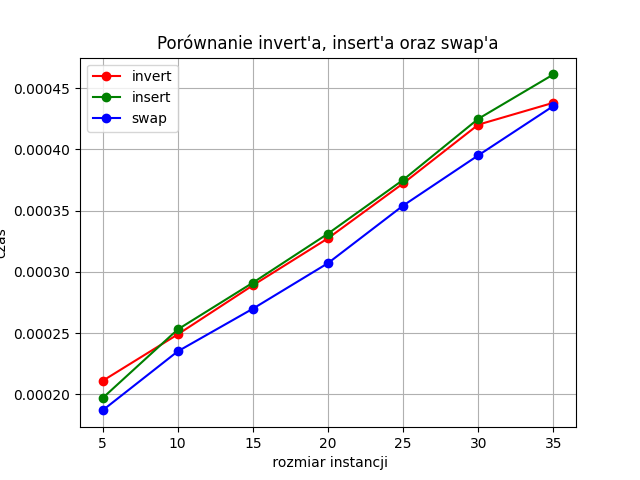
\includegraphics[width=11cm]{./spr2img/Figure_1.png}

    Jak możemy zauważyć, dla wszystkich przeprowadzonych
    przez nas intacji, otocznie \emph{swap} okazało się być
    najelpszym. Pozostałe otoczenia, też nie są źle. Wszystkie
    otoczenia działają w czasie $\mathcal{O}(n)$ i różnią się tylko
    stałą, najmniejszą stałą posiada \emph{swap}

    Poprzednio porównaliśmy jak czas działa dla poszczegołnych otoczeń. Teraz 
    porównamy jak wybór otoczenia wpływa na koszt cyklu dla tych samych 
    intacji.

    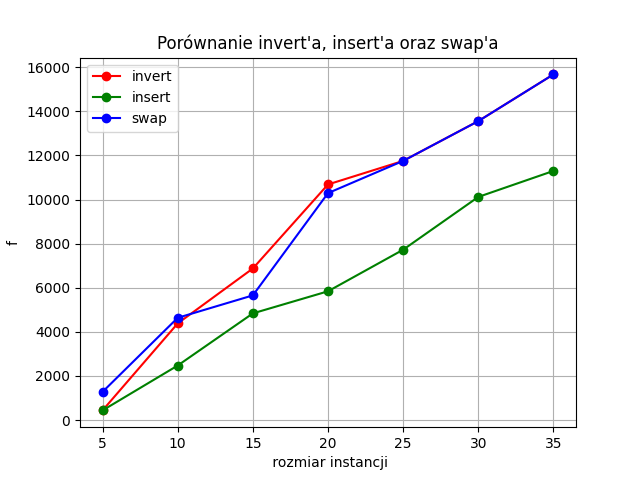
\includegraphics[width=11cm]{./spr2img/Figure_5.png}

    Tym razem \emph{swap} nie był najlepszym wyborem z możliwych przez nas
    zaimplementowanych otoczeń. Teraz najlepszy okazał się \emph{swap}. 
    Wybierając właśnie to otoczenie dla przebadanych instacji, mogliśmy się
    spodziewać funkcji kosztu o najniższej wartośći.

    \section{Czy długość listy Tabu ma znaczenie? }

    Chclieśmy upewnić się, czy zwiększając długość listy
    Tab'u otrzymamy lepszy wynik. tj cykl o najmniejszym koszcie
    w chwili kończenia algortmy. Doskonale wiemy, że jakbyśmy
    zwiększyli sam rozmiar listy tabu to algorytm wykonywał by
    się znacznie dłużej. Dlatego zdecydowaliśmy się, że podzielimy
    wartość (koszt) cyklu na zakończeniu algorytmy przez czas w jakim
    otrzymaliśmy wynik.

    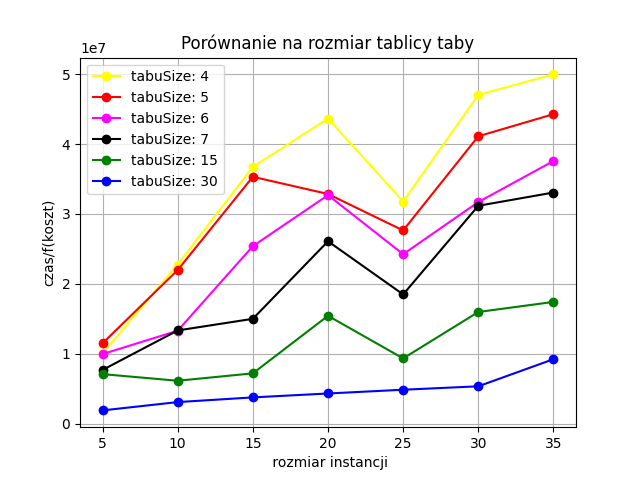
\includegraphics[width=11cm]{./spr2img/Figure_12.png}

    Wyszło, tak jak zakładaliśmy, czyli mimo, że algorytm dłużej
    pracował, (im wieksza liczba tabu, tym dłużej działą), daje lepsze
    wyniki. Zatem warto jest poczekać odpowiednio dłużej aby otrzymać
    lepszy wynik. Pytanie tylko jak długo opłaca się czekać?
    Dla listy tabu długośći 7, obiecujący wynik dostajemy adekwadnie szybko wraz
    z "dobrym" resulatatem. Nie musismy czekać dwa razy dłużej, niż w przypadku
    listy np. dł. 30, a wynik nie różni się znacząco między nimi dwoma.

    \section{Jak decyzja o braku obiecującego rozwiązania z N($\pi$)
            wpływa na koszt?}

    Zaimplemnetowaliśmy wszystkie możliwe kroki, które należy podjąć
    jak wybór obiecującego rozwiązania w otoczeniu są zabronione. Podobnie
    jak na liście zadań wprowadziliśmy następujące oznaczenia. Przez:

    \begin{enumerate}
        \item -> Zakończenie działania algorytmu
        \item -> Stopniowe odrzucanie najstarszych reprezentacji z 
                 listy tabu tak długo aż co najmniej jedno rozwiązanie 
                 nie jest zabronione
        \item -> Dokonanie restartu TS z innego rozwiązania początkowego
        \item -> Przejście do rozwiązań z listy nawrotów, czyli listy 
                 obiecujących rozwiązań tworzonych w trakcie działania algorytmy.
        \item -> Tymczasowe skorzystanie z innego, szerszego otoczenia.
    \end{enumerate}
 
    Z zaimplementowanych przypadków, które należy podjąc przy braku obiecującego
    rozwiązania z N($\pi$), porównaliśmy jak wybór wpływa na funckje kosztu.

    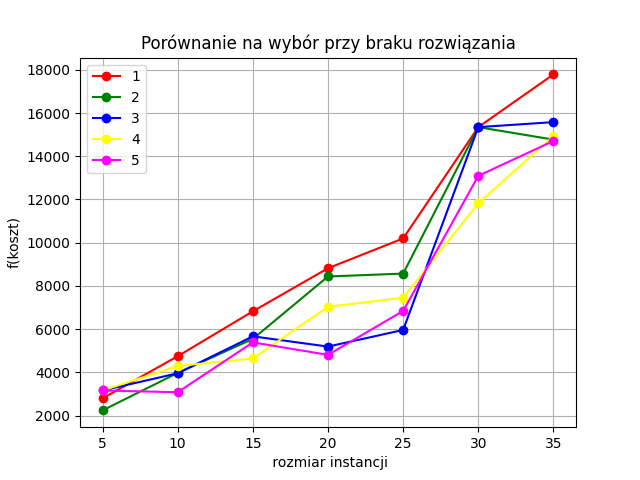
\includegraphics[width=11cm]{./spr2img/Figure_9.png}

    Jak można się było spodziewać, gdy brakuje obiecującego rozwiązania 
    i kończymy z aktulanym najlepiej odkrytymy rozwiązaniem, funckja kosztu
    od niego nie będzie jakaś bardzo obiecująca i praktycznie zawsze będzie
    dawała gorsze rezulaty niż np. użycie listy nawrtotów czy odrzuczanie
    starszych reprezentacji z listy tabu. Dokonanie restatru algorytmy jest
    opartę losowością, cieżko jest stwierdzić czy przynosi zawsze lepszy wynik.
    Możemy cały czas trawiać "dobre" rozwiązania początkowe, które bedą prowadziły
    jednosznaczenie do optymalnego kosztu, a może się zdarzyć że będziemy 
    wybierać przypadki skrajne i wyniki będą dosyć oddalnone od optymalnego 
    rozwiązania.

    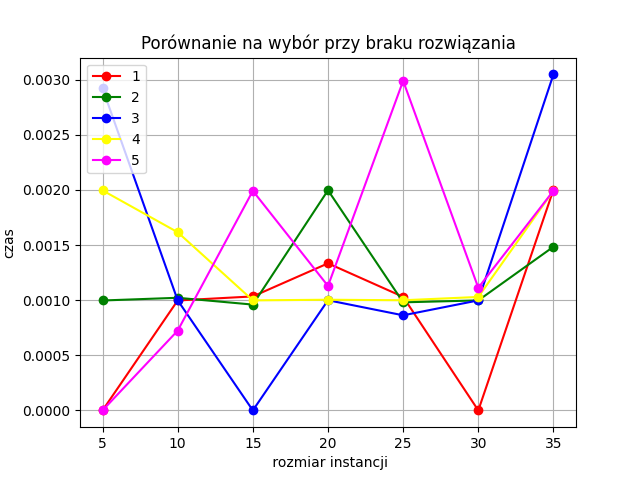
\includegraphics[width=11cm]{./spr2img/Figure_7.png}

    \section{Warunek stopu}

    Zaimplemnetowaliśmy trzy różne warianty zatrzymanai się algorytmu.
    Pierwszy z nich zaznaczono na czerwono na poniższym wykrysie jest ilość ogólnej
    iteracji algoyrtmu. Drugi z koleji, na zielono, ilość iteracji algorytmu, gdzie
    nie znaleźliśmy lepszego rozwiązania, przez k-iteracji. Ostatnim z koleji jest, czas,
    zaznaczony kolorem niebieskim.

    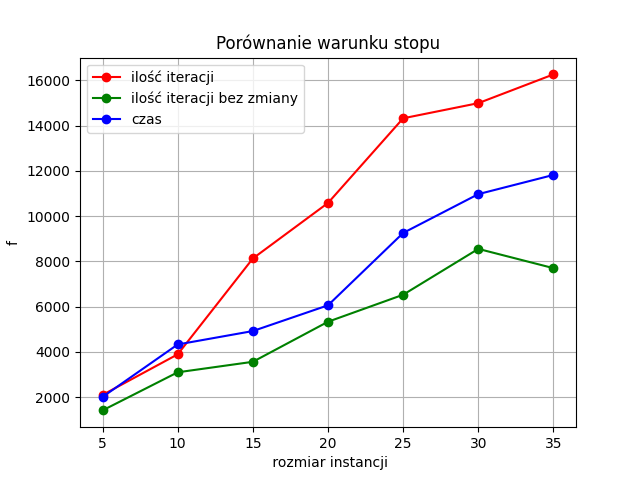
\includegraphics[width=11cm]{./spr2img/Figure_8.png}

    Funckja kosztu dla ogarniczenia samymi iteracjami jest znacząco większa niż liczenie
    iteracji bez zmian. Jest to naturalne zachowanie, wynikające z faktu, że prawie zawsze

    $$I + K = iteracje(iloscBezZmian) > iteracje(zwykle) = I$$

    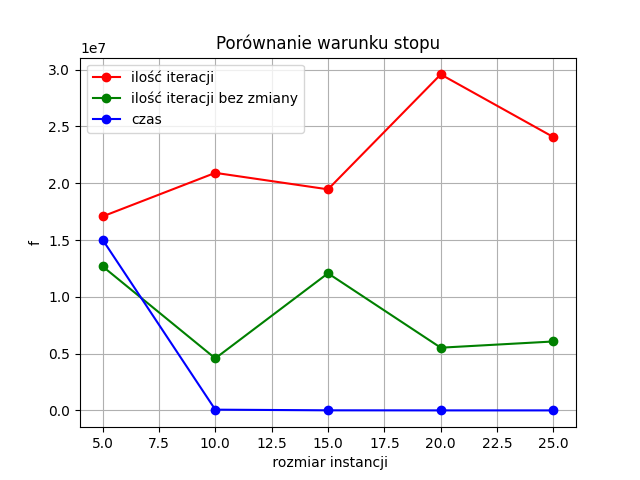
\includegraphics[width=11cm]{./spr2img/Figure_10.png}
    
    Jak można było się spodziewać, ilość iteracji bez zmiany zdecydowanie korzystniej 
    wpływa na funckje kosztu niż sama ilość iteracacji. Teraz porównamy, jak
    warunek stopu wpływa na efektywność optymalnego rozwiązania. Jeżeli wybierzemy odpowiednio duży czas,
    to algorytm będzie tak długo pracował, aż zdajdzie optymalne rozwiązanie. Inaczej jest trochę
    z ograniczeniami na ilośc iteracji. Można było się spodziewać, że w wariancie, gdzie liczby iteracje
    bez zmian, współczynniki  efektywności będzie znacznie lepszy od samego liczenia iteracji.
    Jest to oczywiste, bo iteracje wykonujemy za każdym razem, a iteracji bez zmian wykonamy dodatkowo więcej,
    na koniec działania algorytmu, niż samo liczenie iteracji.

    \section{Złożoność obliczeniowa Tab'u Search}

    Złożonośc obliczeniowa zależy od wielu czynników takich jak:
    rozmiar sąsiedzctwa, wybór otoczenia, długość listy taby.


    Eksperymentalnie wyznaczyliśmy, że algorytm jest $\mathcal{O}(n^2)$

    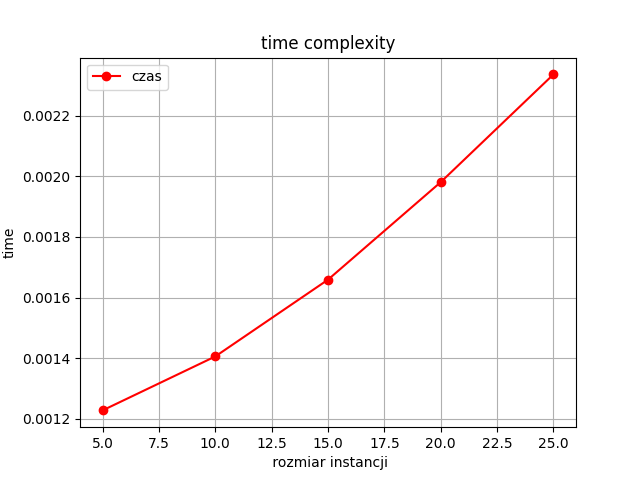
\includegraphics[width=11cm]{./spr2img/Figure_11.png}



\end{document}